% =====================================================================
% VERSION ENSAE, REDUCTION SFE (phase 3, 1er octobre 2026) : chapitre 4, modele frequence-severite.
% Copie a texte constant de chapitres/06_socle_mecaniste.tex.
% Ne changent que les titres et les renvois repares, listes dans
% reduction/phase3.md.
% Lu par main_ensae.tex seul : ne jamais le faire lire par main_institut.tex,
% qui garde chapitres/.
% =====================================================================

\chapter{Modèle fréquence-sévérité}
\label{chap:socle}
\label{part:modele}

\noindent Le calcul distingue trois montants : la perte d'un pilier touché, celle d'un incident
qui peut atteindre plusieurs piliers et la somme des pertes d'une année. Le nombre annuel
d'incidents suit une loi binomiale négative, les pertes élémentaires une loi de Pareto généralisée
au-delà d'un seuil. Leur agrégation dépend de la propagation décrite au chapitre~\ref{chap:cascade}.
La figure~\ref{fig:lecture-architecture} relie ces étapes au quantile annuel qui définit le capital.

% Guide de lecture du calcul ; aucun paramètre ni résultat supplémentaire.
\begin{figure}[H]
\centering
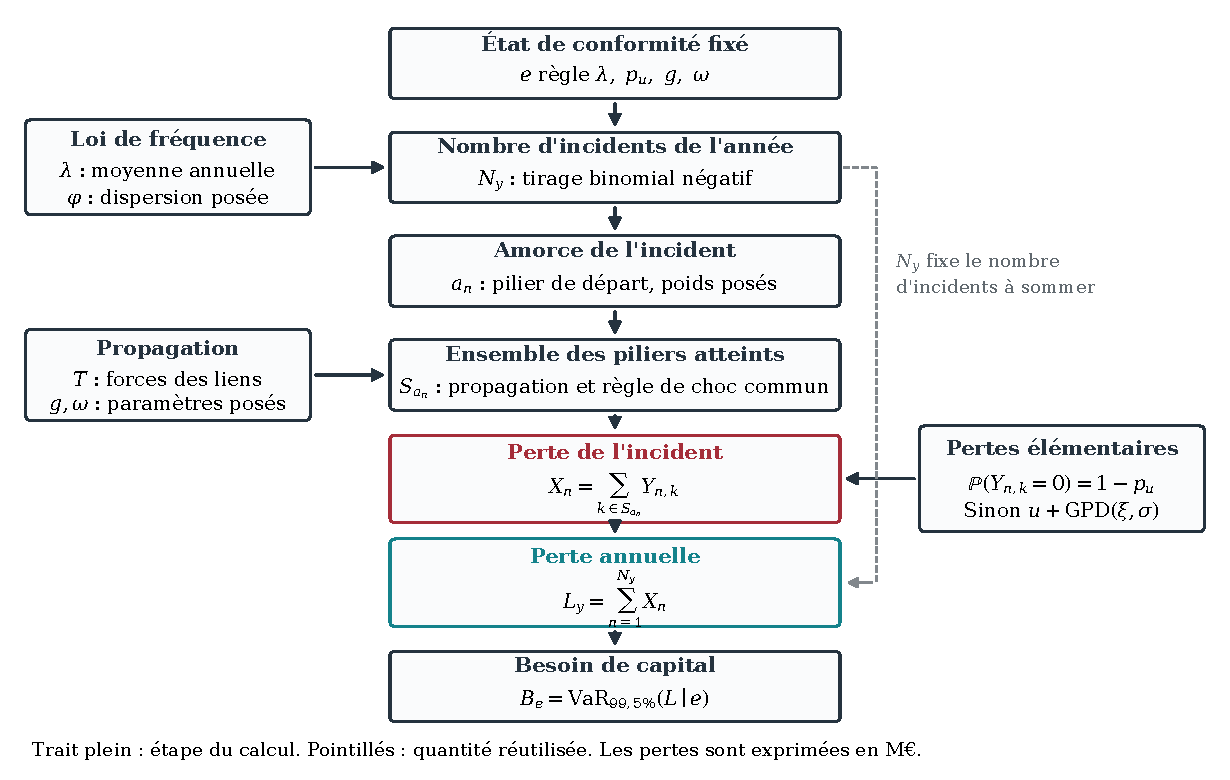
\includegraphics[width=\textwidth]{figures_pedagogie/flux_perte_annuelle.pdf}
\caption{Flux de calcul d'une perte annuelle à état fixé. $y$, $n$ et $k$ indexent l'année simulée, l'incident et le pilier. $u$ est le seuil monétaire ; $\xi$ et $\sigma$ sont la forme et l'échelle de la GPD. Le chapitre~\ref{chap:cascade} détaille la loi des ensembles atteints.}
\label{fig:lecture-architecture}
\end{figure}

Reprenons l'incident de l'introduction : il part de P4 et touche P1 puis P2. Si ses pertes
élémentaires sont $a$, $b$ et $c$, sa contribution à l'année vaut $a+b+c$ sous la règle additive.
Les pertes des autres incidents de cette année s'y ajoutent pour former $L_y$.
Le capital est un quantile des sommes $L_y$ répétées en simulation ; ce n'est pas le quantile
de $a+b+c$ seul. Les branches latérales indiquent les paramètres des étapes. Le tableau~\ref{tab:chaine-calcul}
en précise les sources et le statut, puis indique ce qui change pour une entité.

\begin{table}[htbp]\centering\small
\renewcommand{\arraystretch}{1.18}
\begin{tabularx}{\textwidth}{@{}p{.15\textwidth}>{\raggedright\arraybackslash}X>{\raggedright\arraybackslash}X>{\raggedright\arraybackslash}p{.24\textwidth}@{}}
\toprule
\textbf{Étape} & \textbf{Entrée} & \textbf{Sortie} & \textbf{Statut} \\
\midrule
Données & pertes SAS OpRisk cyber $\times$ finance ; parts Hackmageddon & $\lambda$, $u$, $\xi$, $\sigma$, $p_u$ ; parts $\pi_v$ & estimés (ch.~\ref{chap:donnees} et~\ref{chap:socle}) ; $\pi_v$ cité \\
État & multiplicateurs, détection, $g$, $\omega$ & valeurs des quatre canaux par état & posés (\S\ref{sec:quatre-canaux}) \\
Incident & amorce, matrice $W$, gain $g$ & ensemble atteint, somme des pertes de ses piliers & $W$ posée ; direction non identifiée (ch.~\ref{ch:identifiabilite}) \\
Année & nombre $N_y$, binomiale négative de surdispersion $\varphi$ & charge annuelle $L_y$ & $\varphi$ posé \\
Quantile & charges annuelles simulées & besoin $B=\VaR_{99{,}5\,\%}(L)$ & bruit de simulation publié \\
Entité & panel d'entités, élasticités de fréquence et de sévérité & besoin $B(A)$, cascade indépendante sans choc P4 & élasticité de sévérité estimée ; $b_\lambda$ estimé sur les grandes institutions, extrapolé (\S\ref{sec:ancrage}) \\
\bottomrule
\end{tabularx}
\caption{La chaîne de calcul, étape par étape. Les étapes Incident à Quantile sont celles de la
figure~\ref{fig:lecture-architecture} ; l'étape Entité change de moteur.}
\label{tab:chaine-calcul}
\end{table}


% MIGRÉ depuis memoire/main.tex (plages 787-932, 1492-1667).
% Hiérarchie descendue d'un cran, labels préfixés "soc:".
% RELECTURE FAITE (août 2026). Vérifié : aucune phrase de ce chapitre n'annonce la
% copule de Gumbel ni la variable latente comme LE modèle du mémoire ; la copule
% n'apparaît qu'au chapitre 13 comme axe de comparaison de la bande de modèle.
% Deux ambiguïtés de l'ancien modèle ont été levées ici :
%   (a) l'encadré "deux grilles coexistent" articule vecteur d'attaque et pilier ;
%   (b) l'encadré sur lambda_ref dit explicitement que les 341 de la PRC sont une clé
%       de répartition et n'alimentent PAS le moteur (l'entrée est lambda = 21,6).
% La charge systémique empirique a été corrigée sur la sortie réelle du script 08b
% (a = 0,122 [0,054 ; 0,223] ; phi = 2,24), l'ancien "a ~ 0,30 / phi ~ 3" était faux.
%--------------------------------------------------------------


\section{Théorèmes de l'extrapolation de queue}
% HARNAIS-HORS-SECTION: enonces de theoremes. Les nombres y sont des constantes d'enonce
%   (indices de domaine d'attraction, bornes, dates de publication), aucun n'est calcule
%   par le pipeline ; les valeurs empiriques correspondantes sont verifiees dans les
%   sections de calibration et de validation du meme chapitre.

\begin{theorem}[Fisher--Tippett--Gnedenko]\label{soc:th:ftg}
Soit $(X_i)_{i\ge1}$ indépendantes et de même loi (i.i.d.), de fonction de répartition $F$ et $M_n=\max(X_1,\dots,X_n)$. S'il existe des suites $a_n>0$, $b_n\in\R$ et une loi non dégénérée $H$ telles que $(M_n-b_n)/a_n \xrightarrow{d} H$, alors $H$ est, à un changement d'échelle et de position près, une loi des valeurs extrêmes généralisée (GEV) $H_\xi$. Le signe de $\xi$ détermine le domaine d'attraction : Fréchet ($\xi>0$, queue lourde), Gumbel ($\xi=0$) ou Weibull ($\xi<0$, support borné).
\end{theorem}

\noindent L'approche par maxima de blocs ne retient qu'une observation par bloc. Nous lui
préférons l'approche par dépassement de seuil, qui permet d'exploiter toutes les pertes au-delà d'un
seuil $u$. Celle-ci repose sur le théorème suivant, où
$G_{\xi,\sigma}(y)=1-\left(1+\xi y/\sigma\right)^{-1/\xi}$ désigne la loi de Pareto
généralisée (GPD). L'excès $y=X-u$ est le montant au-dessus du seuil monétaire $u$ ; $\sigma>0$ en règle l'échelle, dans la même unité, et $\xi$ la forme, sans unité. Pour $\xi>0$, la queue décroît en puissance, ce qui définit ici une queue lourde.

\begin{theorem}[Pickands--Balkema--de Haan]\label{soc:th:balkema}
Soit $F$ dans le domaine d'attraction d'une GEV $H_\xi$ (Théorème~\ref{soc:th:ftg}). Alors il existe une fonction $\sigma(u)>0$ telle que la loi des excès converge uniformément vers une GPD lorsque le seuil approche la borne supérieure $x_F$ du support :
\begin{equation}
\lim_{u\to x_F}\ \sup_{0\le y< x_F-u}\bigl|F_u(y)-G_{\xi,\sigma(u)}(y)\bigr|=0,
\end{equation}
où $F_u(y)=\Prob(X-u\le y\mid X>u)$ et $G_{\xi,\sigma}$ est la fonction de répartition de la GPD. L'indice de queue $\xi$ est identique à celui de la GEV limite.
\end{theorem}

\noindent Pour $\xi>0$, la queue est lourde (figure~\ref{fig:domaines-attraction}). La variance de la
sévérité devient infinie dès $\xi\ge 1/2$, et son espérance dès $\xi\ge 1$ \citep{mcneil2015} :
avec $\hat\xi=0{,}595$ ci-dessous, la variance est infinie et l'espérance finie. Les énoncés développés
et les démonstrations figurent à l'annexe~\ref{ann:evt}.

\section{Estimation de l'indice de queue}

% SOURCES-SCRIPTS: 47 63 67

L'estimateur de Hill étant biaisé hors du régime asymptotique strict, nous estimons la GPD par
maximum de vraisemblance sur les $N_u$ excès $y_i$ au-delà du seuil $u$. Pour $\xi \neq 0$, la
log-vraisemblance s'écrit
\begin{equation}
\ell(\xi, \sigma) = -N_u \ln(\sigma) - \left(1 + \frac{1}{\xi}\right) \sum_{i=1}^{N_u} \ln\left(1 + \frac{\xi y_i}{\sigma}\right)
\label{soc:eq:loglik-gpd}
\end{equation}
et se maximise numériquement par Nelder-Mead : c'est l'estimation par maximum de vraisemblance (EMV). L'information de Fisher donne pour
l'indice de queue un intervalle de confiance asymptotique à $90\,\%$ égal à $[0{,}312\,;0{,}878]$,
qui recoupe l'intervalle bootstrap $[0{,}304\,;0{,}831]$.

% Figure ajoutee le 1er octobre 2026, demande de Kelian : tracee par le script 112, et non reprise
% d'un autre memoire. Les indices du panneau (a) et le -0,3 du panneau (b) sont des valeurs
% d'illustration ; seul l'indice calibre est un resultat, lu dans config.py par le script.
\begin{figure}[H]\centering
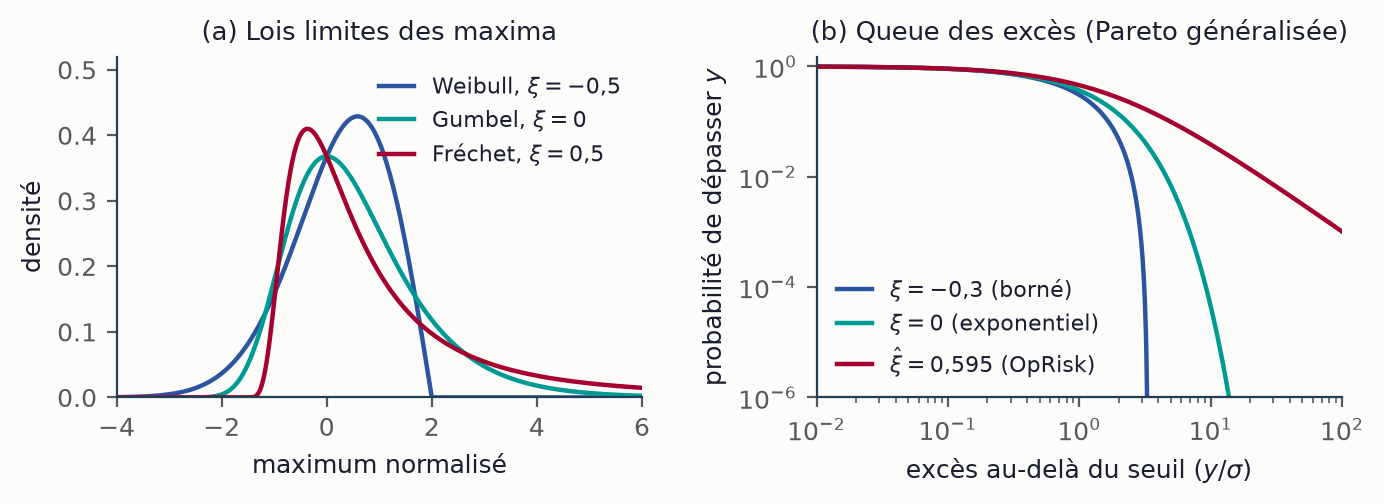
\includegraphics[width=0.95\textwidth]{GEV_domaines_attraction.png}
\caption{Domaines d'attraction des maxima et queue calibrée. (a) Densités des lois des valeurs
extrêmes généralisées de type Weibull ($\xi=-0{,}5$, support borné), Gumbel ($\xi=0$) et Fréchet
($\xi=0{,}5$, queue lourde), valeurs d'illustration. (b) Probabilité qu'un excès dépasse $y$ sous
une loi de Pareto généralisée d'échelle unité, en échelles logarithmiques. Les excès sont bornés
pour $\xi=-0{,}3$, et leur probabilité de dépassement décroît exponentiellement pour $\xi=0$, en
puissance pour l'indice calibré sur OpRisk, $\hat\xi=0{,}595$, qui relève du domaine de Fréchet.}
% SOURCES-SCRIPTS: 112
\label{fig:domaines-attraction}
\end{figure}

En notant $\zeta_u=\Prob(X>u)$ la probabilité de dépassement du seuil (le taux $p_u$ du moteur), on dispose de formes fermées
classiques pour le quantile d'\emph{un} sinistre et sa moyenne de queue \citep{mcneil2015}. Ce
quantile n'est pas un besoin de capital, car celui-ci n'apparaît qu'après agrégation annuelle et
propagation dans la cascade.

\begin{proposition}[Quantile et moyenne de queue d'une sévérité GPD]\label{soc:prop:varestvar}
Sous le modèle POT, pour $\alpha$ tel que $\qsev_\alpha(X)>u$ et $\xi\in(0,1)$ :
\begin{align}
\qsev_\alpha(X) &= \boxed{\,u + \frac{\sigma}{\xi}\left[\left(\frac{1-\alpha}{\zeta_u}\right)^{-\xi}-1\right]\,},\label{soc:eq:var-gpd}\\[4pt]
\qbarsev_\alpha(X) = \E[X\mid X>\qsev_\alpha(X)] &= \boxed{\,\frac{\qsev_\alpha(X)}{1-\xi}+\frac{\sigma-\xi u}{1-\xi}\,}.\label{soc:eq:tvar-gpd}
\end{align}
Lorsque $\xi\ge 1$, l'espérance $\E[X]$ est infinie et $\qbarsev_\alpha$ n'est pas définie.
\end{proposition}

\noindent La calibration OpRisk ($u=20{,}03$, $\sigma=57{,}97$, $\xi=0{,}595$, $\zeta_u=0{,}151$)
donne par \eqref{soc:eq:var-gpd} un quantile de sévérité $\qsev_{99{,}5\%}(X)=663{,}0$~M\euro\ et
par \eqref{soc:eq:tvar-gpd} une moyenne de queue $\qbarsev_{99{,}5\%}(X)=1\,752{,}4$~M\euro. Ces
deux nombres décrivent un sinistre et ne se comparent jamais à un besoin de capital. Celui-ci est
$\VaR_{99{,}5\,\%}(L)$, quantile de la charge annuelle agrégée $L$, de l'ordre de plusieurs milliards
d'euros pour le périmètre financier étudié. Nous réservons $\VaR$ et $\TVaR$ à $L$,
$\qsev$ et $\qbarsev$ à $X$. À $\lambda\simeq21{,}6$ sinistres par an, il faut un quantile
par sinistre de l'ordre de $99{,}98\,\%$ pour atteindre le quantile annuel à $99{,}5\,\%$. Les deux
échelles sont confrontées au \S\ref{sec:ancrage}.
% SOURCES-SCRIPTS: 67

Deux grilles coexistent. Le vecteur d'attaque, comme l'hameçonnage, l'exploitation de
vulnérabilité ou la chaîne d'approvisionnement, décrit comment un incident entre, tandis que le
pilier DORA décrit quel contrôle a cédé. Le vecteur détermine la fréquence d'arrivée des incidents ; le pilier touché en premier suit les parts d'amorce du chapitre~\ref{chap:cascade}. La cascade règle ensuite la propagation entre piliers. Nous ne
supposons aucun appariement entre vecteurs et piliers : les parts $\pi_v$ ne servent qu'à répartir
la fréquence.

\section{Loi de fréquence}

L'entrée du moteur est la fréquence des événements TIC collectés par OpRisk, $\lambda \simeq 21{,}6$
par an pour le périmètre financier étudié ; tous les capitaux de ce périmètre reposent sur elle. Les
calculs d'entité définissent leur fréquence à partir d'un autre panel (\S\ref{sec:ancrage}). Les parts $\pi_v$ de Hackmageddon la répartissent entre vecteurs d'attaque :
$38{,}8\,\%$ hameçonnage, $33{,}8\,\%$ exploitation de vulnérabilités, $15{,}8\,\%$ chaîne
d'approvisionnement, $6{,}3\,\%$ identifiants compromis, $5{,}3\,\%$ autres.

Un défaut de conformité
sur une exigence n'agit ainsi que sur la sous-fréquence $\lambda\,\pi_v$ du vecteur qu'elle atténue.
La fréquence PRC du périmètre financier, $\lambda_{ref} = 341$ notifications américaines par an
($2\,150$ pour la base entière), sans seuil de matérialité, se décompose de la même façon,
$\lambda_v = \lambda_{ref}\,\pi_v$, mais n'entre pas dans le moteur.
% SOURCES-SCRIPTS: 62

Nous avons relu les parts $\pi_v$ sur quatre jeux : premier trimestre 2025, premier semestre 2026,
juillet à octobre 2026 et année 2026 entière, qui recouvre les deux précédents. Notre grille diffère
de celle des décomptes publiés ; les écarts mêlent donc classement et période. Le multiplicateur
non conforme va de $2{,}318$ à $2{,}471$, contre $2{,}487$ publié, soit $6{,}8\,\%$ d'écart au plus.
Cette plage représente $0{,}138$ de celle des fourchettes posées ($1{,}933$ à $3{,}042$) : les
multiplicateurs restent la principale incertitude du canal. Les parts publiées restent des citations
datées. Le champ d'accès initial n'existe que depuis 2025, et la nomenclature MITRE ATT\&CK
introduite en 2026 laisse $46{,}5\,\%$ des vecteurs identifiés de juillet à octobre.
% SOURCES-SCRIPTS: 114 99

La surdispersion signifie que la variance du nombre d'incidents dépasse sa moyenne ($\sigma^2/\mu > 1$, avec $\mu$ la moyenne et $\sigma^2$ la variance du comptage). Pour la représenter, nous modélisons par une loi binomiale négative la fréquence agrégée
$\lambda_{S_x} = \lambda_{\text{C}}\sum_v \pi_v\, m_{v,S_x}$ d'un scénario $S_x$. Ici $\lambda_{\text{C}}\simeq 21{,}6$ est la fréquence de l'état conforme et $m_{v,S_x}$ le multiplicateur posé du vecteur $v$ dans ce scénario, égal à un à l'état conforme. Nous posons $\phi = \sigma^2/\mu = 9{,}2$, constant d'un scénario à l'autre, et le paramètre
$r$ est recalculé :
\begin{equation}
r_{S_x} = \frac{\lambda_{S_x}}{\phi - 1},
\qquad
p_{S_x} = \frac{r_{S_x}}{r_{S_x} + \lambda_{S_x}}.
\end{equation}
Ici $r>0$ est le paramètre de forme du comptage et $p$ son paramètre de probabilité : sa moyenne vaut $r(1-p)/p$, sa variance $r(1-p)/p^2$. Ce $p$ diffère du taux de dépassement $p_u$. La surdispersion en régime de forte dégradation n'est pas observée, faute
d'historique de crise DORA.

Pour un mélange de Poisson, l'indice de dispersion vaut $1+\lambda/r$, si bien qu'il croît avec le
niveau de fréquence auquel on le lit. Il est de $1{,}19$ sur les $14\,944$ cellules firme-année du
panel, de $2{,}24$ sur la série annuelle sectorielle détendancée (IC~$95\,\%$ $[1{,}24\,;5{,}18]$,
dix-huit points), et nous retenons $9{,}20$ dans le moteur.

Cette dernière valeur est un choix de prudence sur la queue de fréquence, pas une calibration. Il
en va de même de la charge systémique $a=0{,}60$ du mélange de la fréquence (supplément), qui dépasse la
borne haute de l'intervalle de la charge empirique $a=0{,}122$ (IC~$95\,\%$ $[0{,}054\,;0{,}223]$).
La charge $a$ est le coefficient du facteur dans le mélange lognormal $\exp(aY-a^2/2)$. Passer du Poisson à la
binomiale négative posée relève le besoin de capital du périmètre financier étudié de $+9\,\%$, la queue
restant déterminée au $99{,}5\,\%$ par la perte unique dominante.
% SOURCES-SCRIPTS: 47 08b 67 41

Les comparaisons annuelles fixent un scénario et leurs tirages sont indépendants entre années.
La distribution des états et leur évolution sont décrites séparément au chapitre~\ref{chap:multietats}.

\section{Loi de sévérité}
\label{soc:sec:severite}

La sévérité élémentaire, tirée pour chaque pilier touché, vaut zéro avec probabilité $1-p_u$, et $u+Y$ sinon, $Y$ suivant la GPD : le corps de la loi sous le seuil est négligé. La perte totale d'un incident est la somme des sévérités élémentaires de ses piliers touchés. La fréquence compte les événements avant ce tirage, ce qui évite de filtrer deux fois.

% SOURCES-SCRIPTS: 07 47 63 67

Les excès suivent la GPD ajustée sur OpRisk au chapitre~\ref{chap:donnees} :
$u = 20{,}0$~M\euro, $86$ excès, $\hat\xi = 0{,}595$, $\hat\sigma = 58{,}0$~M\euro. L'intervalle bootstrap du
quantile de sévérité, $[411\,;\,1037]$~M\euro, représente un facteur~2{,}5
entre les bornes, dû à la seule incertitude de paramètre. Nous plaçons le seuil là où l'indice de
forme quitte la zone $\xi \geq 1$, dans laquelle l'espérance n'existe pas, tout en gardant assez
d'excès pour l'estimation ($n = 86 > 30$). Cet argument ne tient qu'au voisinage du seuil, l'indice
décroissant sur toute la plage (\S\ref{soc:sec:validation}).

\section{Comparer les estimateurs à population fixée}
% SOURCES-SCRIPTS: 129 47 63 67

Le tableau suivant compare les estimateurs sur les mêmes $86$ excès parmi
$570$ pertes de $2000$ à $2026$, au seuil fixé de $20{,}03$~M\euro. Les intervalles percentiles
reposent sur $2\,000$ rééchantillonnages des excès ; ils ne couvrent pas le choix du seuil.
% Généré depuis 129.json par outils/ci/actualiser_complements_hugo.py.
% SOURCES-SCRIPTS: 129
\begin{center}\small
\begin{tabular}{lcc}\toprule Estimateur & $\hat\xi$ & IC bootstrap à $95\,\%$ \\\midrule
EMV & 0{,}595 & [0{,}252 ; 0{,}897] \\
PWM & 0{,}505 & [0{,}254 ; 0{,}622] \\
Hill & 1{,}402 & [1{,}208 ; 1{,}605] \\
Moments & 0{,}863 & [0{,}498 ; 1{,}092] \\
\bottomrule\end{tabular}\end{center}

Hill estime la forme par les logarithmes des pertes rapportées au seuil. L'EMV et les moments pondérés par les probabilités de rang (PWM, \emph{probability-weighted moments}) portent
sur les excès. La ligne Moments utilise les deux premiers moments des logarithmes des pertes
rapportées au seuil. Hors d'une Pareto pure, ces estimateurs ne coïncident pas à seuil fini. Hill et les moments
ne fournissent pas seuls une échelle GPD. Cette réestimation ne remplace pas les constantes gelées.
L'annexe~\ref{ann:evt} conserve le diagnostic historique de Hill.

\section{Adéquation des lois}
\label{soc:sec:validation}

Pour la sévérité, les tracés quantile-quantile et probabilité-probabilité s'alignent sur la
diagonale, et la vie résiduelle moyenne est linéaire au-delà du seuil (figure~\ref{soc:fig:validation}).
Du percentile $85$ au percentile $93$, l'estimation $\hat\xi$ décroît de $0{,}60$ à $0{,}51$ sur
les seuils comptant chacun au moins trente excès. Au percentile $95$, qui n'en compte que $29$, elle
vaut $0{,}34$. Ces valeurs restent dans l'intervalle à $90\,\%$ publié, $[0{,}30\,;0{,}83]$. Sous le
seuil retenu, elle remonte jusqu'à $1{,}03$ et sort de cet intervalle. Ce diagnostic motive le maintien du seuil, sans démontrer qu'un seuil inférieur serait inadmissible.

Sur les mêmes $86$ excès à $20{,}03$~M\euro, les tests de Kolmogorov--Smirnov et d'Anderson--Darling, ce dernier plus sensible aux extrémités, ne rejettent pas la GPD.
Sur $1\,000$ réplications paramétriques avec réestimation, Kolmogorov--Smirnov bilatéral donne
$p=0{,}907$ et Anderson--Darling $p=0{,}983$ ; chaque réplication simule la loi ajustée puis réestime ses paramètres. Le balayage ne démontre pas un seuil optimal. Mesurée par simulation, la couverture
réelle de l'intervalle à $90\,\%$ de $\xi$ est de $87\,\%$, donc l'intervalle est trop
étroit et l'élargir d'environ $8\,\%$ rétablirait le nominal. La sous-couverture concerne l'incertitude de l'estimation ; elle n'établit pas le signe d'un biais du capital. La fréquence gelée et la dérive d'échelle font l'objet de diagnostics distincts (\S\ref{sec:pu-coherence} et \S\ref{soc:sec:backtest}).

Le test du rapport de vraisemblance rejette le Poisson au profit de la binomiale négative (statistique $130{,}5$, $p\approx 10^{-30}$ sur $14\,944$ cellules firme-année), bien que $\Var/\E=1{,}19$ reste proche de un. Ce $p$ traite les cellules comme indépendantes et ignore la dépendance par firme ; le rejet ne calibre pas non plus le facteur $9{,}2$ du moteur.

\begin{figure}[H]\centering
\figover{J3_validation_adequation.png}
\caption{Adéquation du socle. (a-b) Diagrammes quantile-quantile et probabilité-probabilité de la sévérité
contre la GPD ajustée. (c) vie résiduelle moyenne, linéaire au-delà de $u$. (d) stabilité
de $\hat\xi$ au seuil. (e) test d'Anderson-Darling, loi nulle par bootstrap
paramétrique et statistique observée ($p=0{,}98$). (f) adéquation de la fréquence :
la binomiale négative colle aux comptes firme-année, le Poisson rate la queue.}
% SOURCES-SCRIPTS: 47 93 129
\label{soc:fig:validation}
\end{figure}

Une règle de stabilité appliquée à dix percentiles candidats (annexe~\ref{ann:evt}) retient $19{,}32$~M\euro{} contre
$20{,}03$ publiés, avec un quantile supérieur de $1{,}5\,\%$. Le seuil publié est compatible avec ces diagnostics ; une p-value élevée n'établit pas son optimalité.
La règle la plus permissive descendrait à $15{,}53$~M\euro{} et donnerait un quantile de sévérité
supérieur de $10{,}3\,\%$.

Retirer chaque excès à son tour laisse le quantile dans l'intervalle publié ; le maximum,
$1\,380$~M\euro, le déplace de $-16{,}0\,\%$. Retirer les trois plus grosses pertes le fait sortir
par le bas ; en retirer cinq le ramène de $662{,}8$ à $326{,}8$~M\euro. Le quantile dépend donc de
quelques pertes. Ce diagnostic ne valide pas le niveau du capital.
% SOURCES-SCRIPTS: 106 41

\section{Backtest hors échantillon}
\label{soc:sec:backtest}

Pour chaque année d'origine, nous ajustons les deux lois sur les seules observations antérieures et
évaluons la prévision de l'année suivante, puis l'origine avance d'un an. La fenêtre va de $2004$ à $2025$
($539$ incidents, douze années notées), car avant $2004$ la base compte de un à neuf incidents par
an, et $2026$ n'en compte que cinq. Le seuil est ré-estimé sur chaque échantillon d'apprentissage
par la règle du percentile $85$.

L'intervalle de prévision à $90\,\%$ du nombre annuel d'incidents couvre $11$ années sur $12$ sous la binomiale négative,
contre $9$ sous le Poisson ; son log-score cumulé gagne $3{,}054$ nats. Ce résultat ne valide
pas la surdispersion posée dans le moteur. La forme GPD n'est pas rejetée ($p=0{,}4087$), mais le test de Kupiec, qui compare les nombres de dépassements observé et attendu, rejette la couverture des quantiles de sévérité à $99\,\%$ ($p=0{,}0078$) et
$99{,}5\,\%$ ($p=0{,}0140$). La dérive d'échelle estimée, $3{,}40\,\%$ par an, reste non
significative ($p=0{,}1786$). Le niveau de charge annuelle est aussi rejeté sur les dernières
années notées, sans cause établie. L'annexe~\ref{sec:ann-backtest} détaille ces tests et l'effet
conditionnel d'une échelle variable ; le registre des limites (\S\ref{sec:pu-coherence}) en conserve
la portée, sans changer le capital publié.
% SOURCES-SCRIPTS: 89 90 91 102

Détecter un doublement du taux de dépassement avec $80\,\%$ de puissance demanderait $1\,811$
années à $99{,}5\,\%$, $905$ à $99\,\%$ et $78$ à $90\,\%$. Douze années ne permettent donc
pas de valider le quantile de capital.

\subsection{Comparaison à des modèles d'apprentissage statistique}
\label{soc:sec:benchmark-apprentissage}

Aucun modèle à caractéristiques n'améliore la tendance temporelle seule avec un intervalle
à $90\,\%$ excluant zéro. Le boosting obtient le meilleur log-score ; son gain de $0{,}0193$
a pour intervalle $[-0{,}0371\,;+0{,}0571]$, par bootstrap des années évaluées.

Nous appliquons le script \texttt{131} aux $570$ pertes, dont $86$ au-dessus de $20{,}03$~M\euro,
en excluant les cinq pertes de l'année $2026$, incomplète. L'évaluation en origine glissante,
de $2014$ à $2025$, porte sur $280$ pertes, dont $60$ dépassements. La cible est conditionnelle à l'enregistrement d'une perte ;
elle n'est pas une fréquence annuelle d'incident.

Nous comparons un taux constant (M0), une régression logistique sur l'année (M1), une régression
logistique pénalisée $L_2$ (M2) et un boosting d'arbres de gradient (M3). M2 et M3 ajoutent le métier
bâlois, la région de domicile, la catégorie d'événement et le logarithme des actifs à l'année.
La pénalisation $L_2$ limite la taille des coefficients ; le boosting combine des arbres successifs
pour corriger leurs erreurs. Leurs réglages, appelés hyperparamètres, sont fixés avant l'évaluation.
Les log-scores moyens, plus élevés quand
la prévision est meilleure, sont :
\begin{center}\small
\begin{tabular}{@{}lrrrr@{}}
\toprule
Modèle & M0 & M1 & M2 & M3 \\
\midrule
Log-score & $-0{,}5605$ & $-0{,}5214$ & $-0{,}5436$ & $-0{,}5021$ \\
\bottomrule
\end{tabular}
\end{center}
Le bootstrap par années ne distingue pas non plus la tendance M1 du taux constant M0.
L'information financière est postérieure à l'événement pour $37\,\%$ des pertes. Masquer les actifs
postérieurs à l'année de l'événement laisse l'intervalle du gain du boosting inclure zéro.

La GPD DX, dont l'échelle ajoute le logarithme des actifs et la catégorie à la tendance,
attribue une densité nulle à une perte observée.
Sa forme négative borne le support, ensemble des pertes possibles sous la loi, sous cet excès.
Sur les $59$ autres excès, son écart de log-score contre l'échelle en tendance seule (D) vaut
$-0{,}0645$, d'intervalle à $90\,\%$ $[-0{,}1738\,;+0{,}0691]$. Cette moyenne conditionnelle
omet l'échec de support.

Ces résultats restent compatibles avec la queue commune retenue au \S\ref{sec:profilage-variables}.
Dans cette chaîne, l'extrapolation des montants extrêmes reste confiée à la GPD ; les classifieurs
n'estiment que le dépassement du seuil. Le registre n'observe pas l'exposition, et $35$ pertes
notées viennent d'une firme déjà présente dans l'apprentissage. Les intervalles ne reposent
que sur douze blocs annuels.
% SOURCES-SCRIPTS: 131

Les lois ajustées permettent de compter les incidents et de tirer leurs pertes élémentaires.
Pour l'exemple P4$\to$P1$\to$P2, elles fournissent les coûts $a$, $b$ et $c$ ; l'atteinte de ces
piliers relève de la propagation (chapitre~\ref{chap:cascade}).
